\documentclass[11pt,letterpaper]{article}
\usepackage[lmargin=1in,rmargin=1in,tmargin=1in,bmargin=1in]{geometry}
\usepackage{../style/homework}
\usepackage{../style/commands}
\setbool{quotetype}{false} % True: Side; False: Under
\setbool{hideans}{false} % Student: True; Instructor: False

% -------------------
% Content
% -------------------
\begin{document}

\homework{7: Due 01/13}{You guys I'm, like, really smart now. You don’t even know. You could ask me, `Kelly, what’s the biggest company in the world?' And I’d be like, `blah blah blah, blah blah blah blah blah blah.' Giving you the exact right answer.}{Kelly Kapoor, The Office}

% Problem 1
\problem{10} Sketch the function $f(x)= (x + 3)^2 - 5$. 
	\[
	\fbox{
	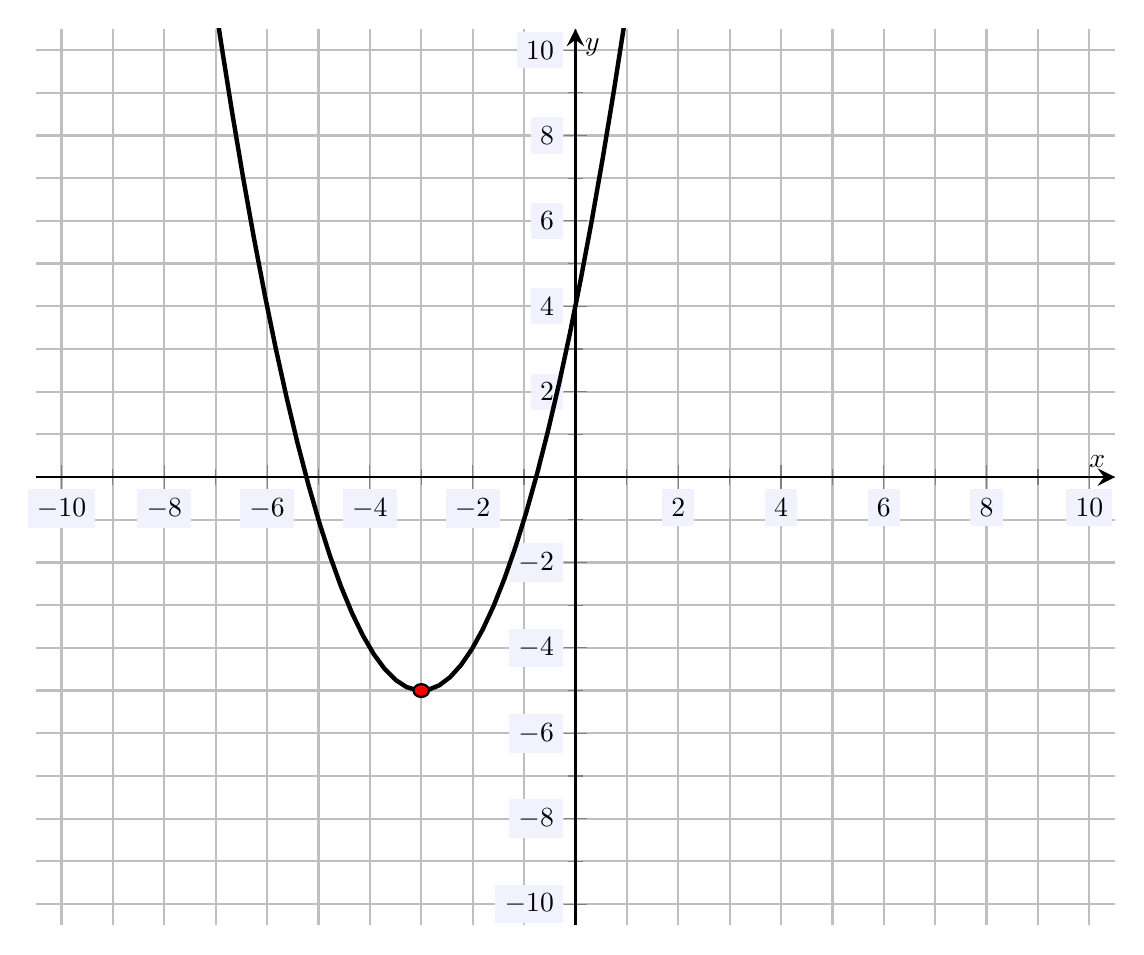
\begin{tikzpicture}[scale=2,every node/.style={scale=0.5}]
	\begin{axis}[
	grid=both,
	axis lines=middle,
	ticklabel style={fill=blue!5!white},
	xmin= -10.5, xmax=10.5,
	ymin= -10.5, ymax=10.5,
	xtick={-10,-8,-6,-4,-2,0,2,4,6,8,10},
	ytick={-10,-8,-6,-4,-2,0,2,4,6,8,10},
	minor tick = {-10,-9,...,10},
	xlabel=\(x\),ylabel=\(y\),
	]
	\addplot[thick, domain= -10.5:10.5, samples=100] ({x},{(x + 3)^2 - 5});
	\draw[fill=red] (-3, -5) circle (0.15);
	\end{axis}
	\end{tikzpicture}
	}
	\] \pspace

Because this quadratic function is in vertex form, we see that the vertex is $(-3, -5)$. Because $a= 1 > 0$, the quadratic function opens upwards, i.e. is concave up or convex. We can then sketch the quadratic function as above. 



\newpage



% Problem 2
\problem{10} Sketch the function $f(x)= 8 - 2(x - 6)^2$. 
	\[
	\fbox{
	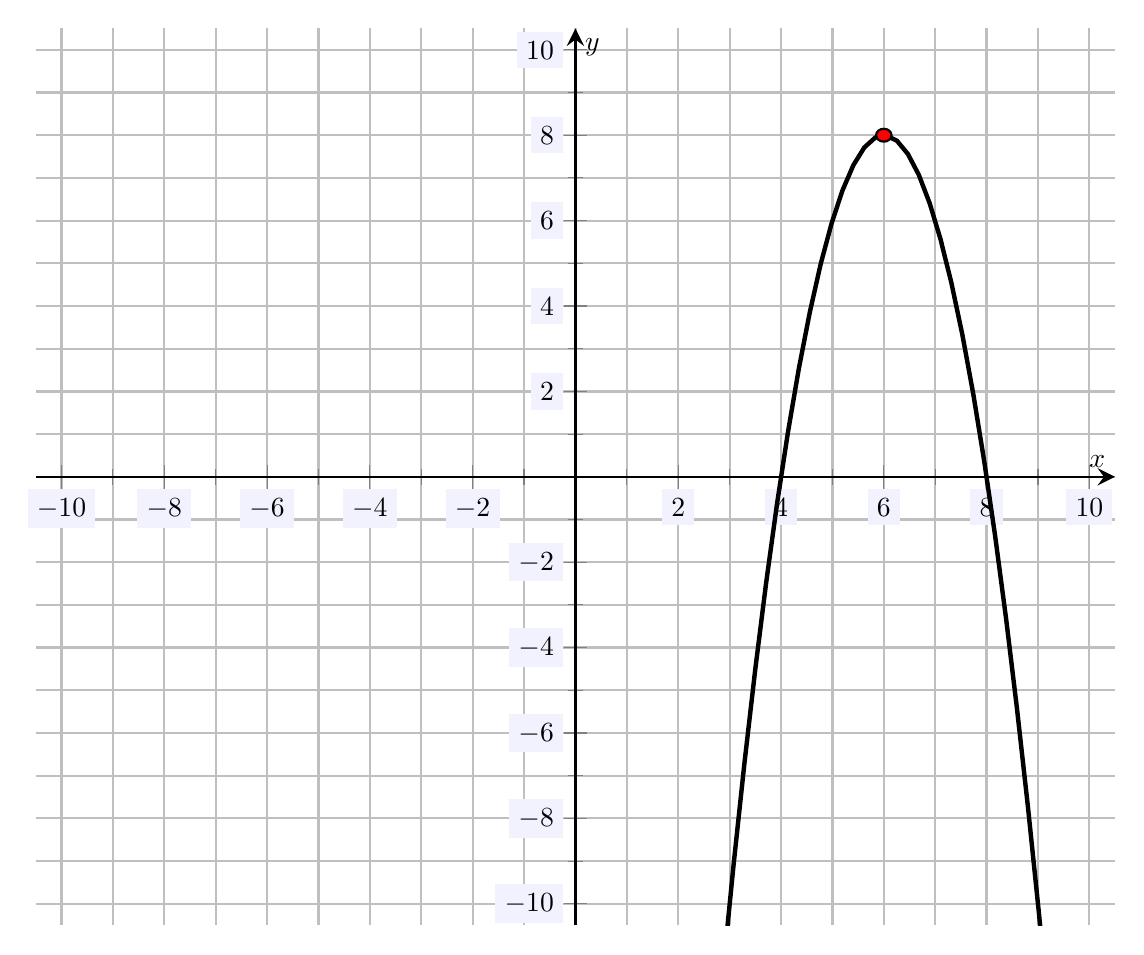
\begin{tikzpicture}[scale=2,every node/.style={scale=0.5}]
	\begin{axis}[
	grid=both,
	axis lines=middle,
	ticklabel style={fill=blue!5!white},
	xmin= -10.5, xmax=10.5,
	ymin= -10.5, ymax=10.5,
	xtick={-10,-8,-6,-4,-2,0,2,4,6,8,10},
	ytick={-10,-8,-6,-4,-2,0,2,4,6,8,10},
	minor tick = {-10,-9,...,10},
	xlabel=\(x\),ylabel=\(y\),
	]
	\addplot[thick, domain= -10.5:10.5, samples=100] ({x},{8 - 2*(x - 6)^2});
	\draw[fill=red] (6, 8) circle (0.15);
	\end{axis}
	\end{tikzpicture}
	}
	\] \pspace

Because this quadratic function is in vertex form, we see that the vertex is $(6, 8)$. Because $a= -2 < 0$, the quadratic function opens downwards, i.e. is concave down or concave. We can then sketch the quadratic function as above. 



\newpage



% Problem 3
\problem{10} Sketch the function $f(x)= x^2 - 10x + 16$.
	\[
	\fbox{
	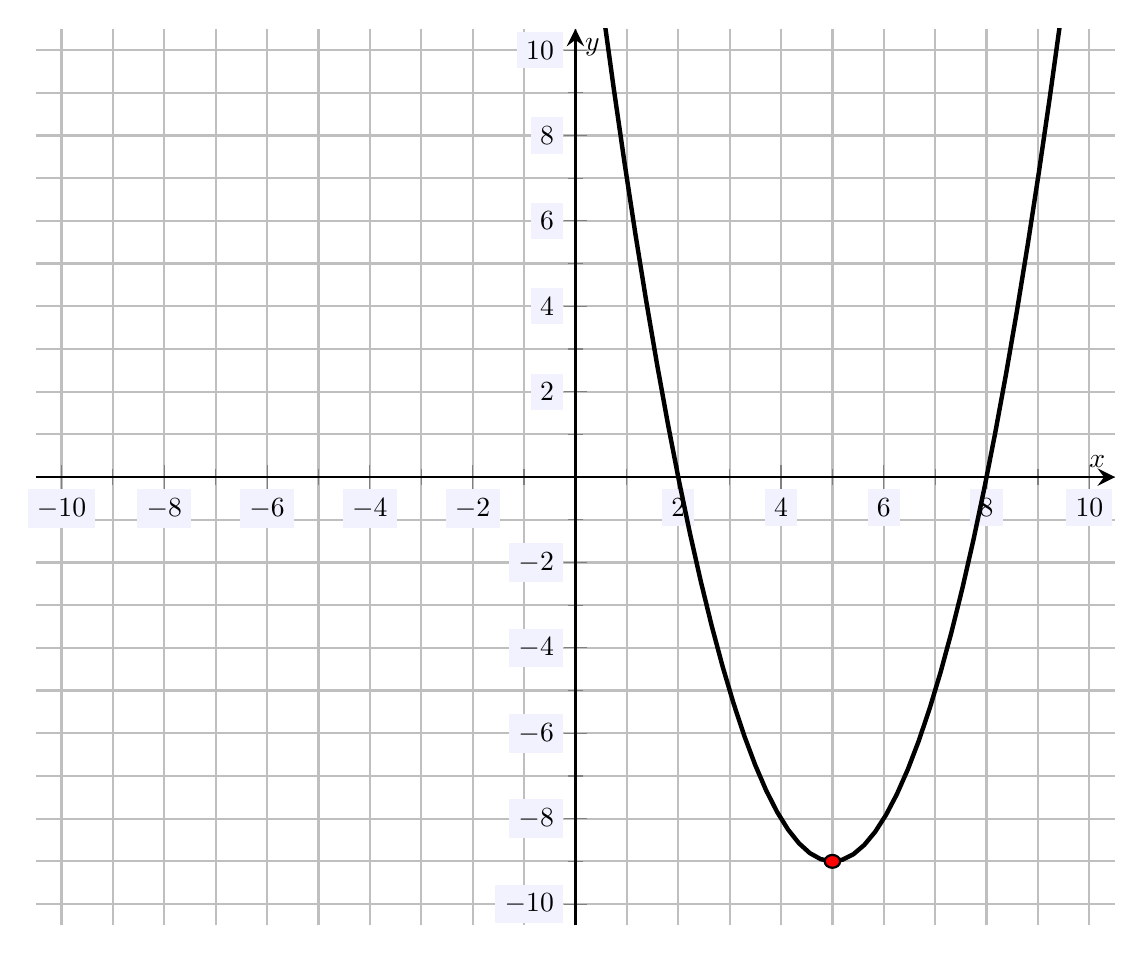
\begin{tikzpicture}[scale=2,every node/.style={scale=0.5}]
	\begin{axis}[
	grid=both,
	axis lines=middle,
	ticklabel style={fill=blue!5!white},
	xmin= -10.5, xmax=10.5,
	ymin= -10.5, ymax=10.5,
	xtick={-10,-8,-6,-4,-2,0,2,4,6,8,10},
	ytick={-10,-8,-6,-4,-2,0,2,4,6,8,10},
	minor tick = {-10,-9,...,10},
	xlabel=\(x\),ylabel=\(y\),
	]
	\addplot[thick, domain= -10.5:10.5, samples=100] ({x},{x^2 - 10*x + 16});
	\draw[fill=red] (5, -9) circle (0.15);
	\end{axis}
	\end{tikzpicture}
	}
	\] \pspace

We can find a table of values to sketch the function, i.e.
	\begin{table}[!ht]
	\centering
	\begin{tabular}{r||rrrrrrrrrrr}
	$x$ & $0$ & $1$ & $2$ & $3$ & $4$ & $5$ & $6$ & $7$ & $8$ & $9$ & $10$ \\ \hline
	$f(x)$ & $16$ & $7$ & $0$ & $-5$ & $-8$ & $-9$ & $-8$ & $-5$ & $0$ & $7$ & $16$
	\end{tabular}
	\end{table}
Alternatively, we can complete the square to put the quadratic function into vertex form:
	\[
	f(x)= x^2 - 10x + 16= x^2 - 10x + \left( \dfrac{-10}{2} \right)^2 - \left( \dfrac{-10}{2} \right)^2 + 16= x^2 - 10x + 25 - 25 + 16= (x - 5)^2 - 9
	\]
We then see the vertex is $(5, -9)$ and because $a= 1 > 0$, the parabola opens upwards, i.e. is concave up or convex. We can then sketch the function as above. 



\newpage



% Problem 4
\problem{10} Find the vertex form of $y= -2x^2 + 12x - 13$ by completing the square. \pspace

\sol First, we factor our the $-2$, which gives us $y= -2(x^2 - 6x + 13/2)$. The $x$ coefficient is $-6$. We have $(\frac{1}{2} \cdot -6)^2= (-3)^2= 9$. Then we have\dots
	\[
	\begin{aligned}
	y&= -2x^2 + 12x - 13 \\[0.3cm]
	y&= -2 \left( x^2 - 6x + \dfrac{13}{2} \right) \\[0.3cm]
	y&= -2 \left( x^2 - 6x + \left( \dfrac{-6}{2} \right)^2 - \left( \dfrac{-6}{2} \right)^2 + \dfrac{13}{2} \right) \\[0.3cm]
	y&= -2 \left( x^2 - 6x + 9 - 9 + \dfrac{13}{2} \right) \\[0.3cm]
	y&= -2 \left( (x - 3)^2 - \dfrac{5}{2} \right) \\[0.3cm]
	y&= -2(x - 3)^2 + 5 \\[0.3cm]
	y&= 5 - 2(x - 3)^2
	\end{aligned}
	\]



\newpage



% Problem 5
\problem{10} Find the vertex form of $y= x^2 - 12x + 48$ by the `evaluation method.' \pspace 

\sol A general quadratic function has the form $y= ax^2 + bx + c$. For this quadratic function, $a= 1$, $b= -12$, and $c= 48$. We know the vertex occurs at $x= \dfrac{-b}{2a}= \dfrac{-(-12)}{2(1)}= \dfrac{12}{2}= 6$. The corresponding $y$-value is\dots
	\[
	y(6)= 6^2 - 12(6) + 48= 36 - 72 + 48= -36 + 48= 12
	\]
Therefore, the vertex is $(6, 12)$. Therefore, the vertex form is\dots
	\[
	y= 1 \cdot (x - 6)^2 + 12= (x - 6)^2 + 12
	\]



\newpage



% Problem 6
\problem{10} Showing all your work, factor $x^2 + 14x - 51$. \pspace

\sol 
	\begin{table}[!ht]
	\centering
	\underline{\bfseries 51} \pvspace{0.2cm}
	\begin{tabular}{rr}
	$1 \cdot -51$ & $-50$ \\
	$-1 \cdot 51$ & $50$ \\
	$3 \cdot -17$ & $-14$ \\ \hline
	\multicolumn{1}{|r}{$-3 \cdot 17$} & \multicolumn{1}{r|}{$14$} \\ \hline
	\end{tabular}
	\end{table}

Therefore,
	\[
	x^2 + 14x - 51= (x - 3)(x + 17)
	\]



\newpage



% Problem 7
\problem{10} Showing all your work, factor $x^2 + 10x - 56$. \pspace

\sol 
	\begin{table}[!ht]
	\centering
	\underline{\bfseries 56} \pvspace{0.2cm}
	\begin{tabular}{rr}
	$1 \cdot -56$ & $-55$ \\
	$-1 \cdot 56$ & $55$ \\
	$2 \cdot -28$ & $-26$ \\
	$-2 \cdot 28$ & $26$ \\
	$4 \cdot -14$ & $-10$ \\ \hline
	\multicolumn{1}{|r}{$-4 \cdot 14$} & \multicolumn{1}{r|}{$10$} \\ \hline
	$7 \cdot -8$ & $-1$ \\
	$-7 \cdot 8$ & $1$ 
	\end{tabular}
	\end{table}

Therefore,
	\[
	x^2 + 10x - 56= (x - 4)(x + 14)
	\]



\newpage



% Problem 8
\problem{10} Showing all your work, factor $3x^2 + 7x - 20$. \pspace

\sol 
	\begin{table}[!ht]
	\centering
	\underline{\bfseries 20} \pvspace{0.1cm}
	\begin{tabular}{c}
	$1 \cdot -20$ \\
	$-1 \cdot 20$ \\
	$2 \cdot -10$ \\
	$-2 \cdot 10$ \\
	$4 \cdot -5$ \\
	$-4 \cdot 5$
	\end{tabular}
	\end{table}

Then as $3= 1 \cdot 3$, we have\dots
	\[
	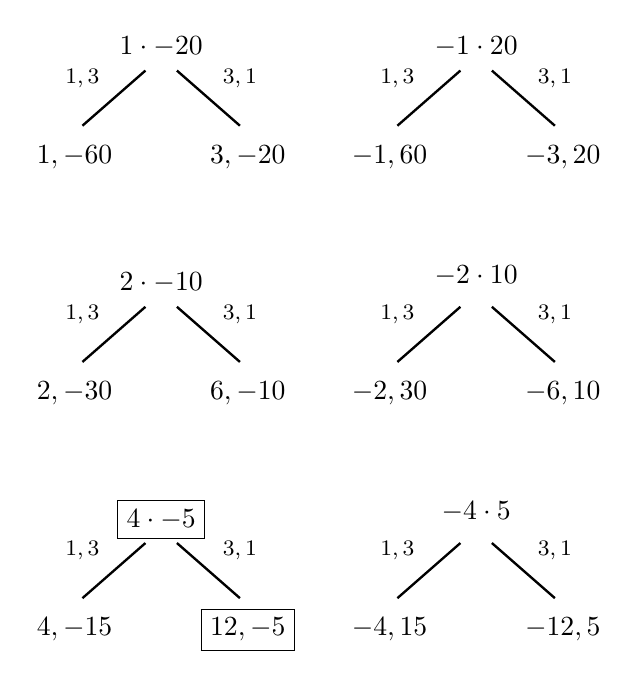
\begin{tikzpicture}
	\node at (0,0) {$1 \cdot -20$};
	\node at (-1.0,-0.4) {\footnotesize$1, 3$};
	\draw[line width=0.03cm,label={1}] (-0.2,-0.3) -- (-1,-1);
	\node at (-1.1,-1.4) {$1, -60$};
	\node at (1.0,-0.4) {\footnotesize$3,1$};
	\draw[line width=0.03cm] (0.2,-0.3) -- (1,-1);
	\node at (1.1,-1.4) {$3, -20$};	
	
	\tikzset{shift={(4,0)}}

	\node at (0,0) {$-1 \cdot 20$};
	\node at (-1.0,-0.4) {\footnotesize$1, 3$};
	\draw[line width=0.03cm,label={1}] (-0.2,-0.3) -- (-1,-1);
	\node at (-1.1,-1.4) {$-1, 60$};
	\node at (1.0,-0.4) {\footnotesize$3, 1$};
	\draw[line width=0.03cm] (0.2,-0.3) -- (1,-1);
	\node at (1.1,-1.4) {$-3, 20$};

	\tikzset{shift={(-4,-3)}}

	\node at (0,0) {$2 \cdot -10$};
	\node at (-1.0,-0.4) {\footnotesize$1, 3$};
	\draw[line width=0.03cm,label={1}] (-0.2,-0.3) -- (-1,-1);
	\node at (-1.1,-1.4) {$2, -30$};
	\node at (1.0,-0.4) {\footnotesize$3, 1$};
	\draw[line width=0.03cm] (0.2,-0.3) -- (1,-1);
	\node at (1.1,-1.4) {$6, -10$};

	\tikzset{shift={(4,0)}}

	\node at (0,0.1) {$-2 \cdot 10$};
	\node at (-1.0,-0.4) {\footnotesize$1, 3$};
	\draw[line width=0.03cm,label={1}] (-0.2,-0.3) -- (-1,-1);
	\node at (-1.1,-1.4) {$-2, 30$};
	\node at (1.0,-0.4) {\footnotesize$3, 1$};
	\draw[line width=0.03cm] (0.2,-0.3) -- (1,-1);
	\node at (1.1,-1.4) {$-6, 10$};
	
	\tikzset{shift={(-4,-3)}}

	\node at (0,0) {\framebox{$4 \cdot -5$}};
	\node at (-1.0,-0.4) {\footnotesize$1, 3$};
	\draw[line width=0.03cm,label={1}] (-0.2,-0.3) -- (-1,-1);
	\node at (-1.1,-1.4) {$4, -15$};
	\node at (1.0,-0.4) {\footnotesize$3, 1$};
	\draw[line width=0.03cm] (0.2,-0.3) -- (1,-1);
	\node at (1.1,-1.4) {\framebox{$12, -5$}};

	\tikzset{shift={(4,0)}}

	\node at (0,0.1) {$-4 \cdot 5$};
	\node at (-1.0,-0.4) {\footnotesize$1, 3$};
	\draw[line width=0.03cm,label={1}] (-0.2,-0.3) -- (-1,-1);
	\node at (-1.1,-1.4) {$-4, 15$};
	\node at (1.0,-0.4) {\footnotesize$3, 1$};
	\draw[line width=0.03cm] (0.2,-0.3) -- (1,-1);
	\node at (1.1,-1.4) {$-12, 5$};
	\end{tikzpicture}
	\]

Therefore, 
	\[
	3x^2 + 7x - 20= (3x - 5)(x + 4)
	\]



\newpage



% Problem 9
\problem{10} Consider the quadratic function $f(x)= x^2 + 14x + 39$.
        \begin{enumerate}[(a)]
        \item Determine if the parabola opens upwards or downwards.
        \item Is the parabola convex or concave?
        \item Does the parabola have a maximum or minimum? 
        \item Find the vertex and axis of symmetry. 
        \item Find the maximum/minimum value of $f(x)$. 
        \end{enumerate} \pspace

\sol
\begin{enumerate}[(a)]
\item Because $a= 1 > 0$, this quadratic function opens upwards, i.e. is concave up. \pspace

\item Because the parabola opens upwards, we know that the function is convex. \pspace

\item Because the parabola opens upwards, the quadratic function has a minimum. \pspace

\item The vertex occurs when $x= -\frac{b}{2a}= -\frac{14}{2(1)}= -7$. But then the axis of symmetry is $x= -7$. We have
	\[
	y(-7)= (-7)^2 + 14(-7) + 39= 49 - 98 + 39= -49 + 39= -10
	\]
Therefore, the vertex is $(-7, -10)$. Alternatively, putting the parabola in vertex form:
	\[
	\begin{aligned}
	y&= x^2 + 14x + 39 \\[0.3cm]
	y&= x^2 + 14x + (49 - 49) + 39 \\[0.3cm]
	y&= (x^2 + 14x + 49) - 49 + 39 \\[0.3cm]
	y&= (x + 7)^2 - 10 
	\end{aligned}
	\]
we can easily see that the vertex is $(-7, -10)$ and that the axis of symmetry is $x= -7$. \pspace
 
\item Because the parabola opens upwards, the parabola has a minimum. The minimum occurs at the vertex. The vertex is $(-7, -10)$. Therefore, the minimum value is $-10$.  
\end{enumerate}



\newpage



% Problem 10
\problem{10} Consider the quadratic function $f(x)= -2x^2 + 4x + 3$.
        \begin{enumerate}[(a)]
        \item Determine if the parabola opens upwards or downwards.
        \item Is the parabola convex or concave?
        \item Does the parabola have a maximum or minimum? 
        \item Find the vertex and axis of symmetry. 
        \item Find the maximum/minimum value of $f(x)$. 
        \end{enumerate} \pspace

\sol
\begin{enumerate}[(a)]
\item Because $a= -2 < 0$, this quadratic function opens downwards, i.e. is concave down. \pspace

\item Because the parabola opens downwards, we know that the function is concave. \pspace

\item Because the parabola opens downwards, the quadratic function has a maximum. \pspace

\item The vertex occurs when $x= -\frac{b}{2a}= -\frac{4}{2(-2)}= 1$. But then the axis of symmetry is $x= 1$. We have
	\[
	y(1)= -2(1^2) + 4(1) + 3= -2 + 4 + 3= 2 + 3= 5
	\]
Therefore, the vertex is $(1, 5)$. Alternatively, putting the parabola in vertex form:
	\[
	\begin{aligned}
	y&= -2x^2 + 4x + 3 \\[0.3cm]
	y&= -2 \left(x^2 - 2x - \frac{3}{2} \right) \\[0.3cm]
	y&= -2 \left(x^2 - 2x + (1 - 1) - \frac{3}{2} \right) \\[0.3cm] 
	y&= -2 \left( (x^2 - 2x + 1) - 1 - \frac{3}{2} \right) \\[0.3cm] 
	y&= -2 \left( (x - 1)^2 - \frac{5}{2} \right) \\[0.3cm] 
	y&= -2(x - 1)^2 + 5
	\end{aligned}
	\]
we can easily see that the vertex is $(1, 5)$ and that the axis of symmetry is $x= 1$. \pspace
 
\item Because the parabola opens downwards, the parabola has a maximum. The maximum occurs at the vertex. The vertex is $(1, 5)$. Therefore, the maximum value is $5$.  
\end{enumerate}


\end{document}